\documentclass{beamer}

\usetheme[progressbar=frametitle]{metropolis}
\setbeamertemplate{frame numbering}[fraction]
\useoutertheme{metropolis}
\useinnertheme{metropolis}
\usefonttheme{metropolis}
\usecolortheme{spruce}
\setbeamercolor{background canvas}{bg=white}
\definecolor{mygreen}{rgb}{.125,.5,.25}
\usecolortheme[named=mygreen]{structure}

\usepackage{amsmath}
\usepackage{pst-node}
%\usepackage{tikz,lipsum,lmodern}
\usepackage{tcolorbox}
\usepackage{multicol}
\usepackage{graphicx}
\graphicspath{{C:/Users/LAB5892A/Desktop/outgoing/figures/EKF/}}

\setcounter{MaxMatrixCols}{20}
\title{SLAM For Autonomous Ground Vehicles}
\subtitle{Attached 1}
\author{Li Hong Rong}
%\institute{\large\textbf{Learning Outcomes}:\\[6pt]Kalmen filter, extended Kalman filter, algorithm on SLAM}
\date{}
\begin{document}
\metroset{block=fill}
\begin{frame}
\titlepage
\end{frame}


\begin{frame}[t]{Overall}
\begin{itemize}
\item Research Motivation
\item Literature Reviews
\item Research Approaches
\item Progress
\item Application
\end{itemize}
\end{frame}

\begin{frame}[t]{Research motivation}
\begin{enumerate}[1.]
\item REDUCED ACCIDENTS\\
\vspace{0.5pt}
\begin{tcolorbox}[colback=green!5!white,colframe=green!75!black]
Self-driving cars are projected to reduce traffic deaths by 90 percent, saving 30,000 lives a year
\end{tcolorbox}
\item REDUCED TRAFFIC CONGESTION\\
\vspace{0.5pt}
\begin{tcolorbox}[colback=green!5!white,colframe=green!75!black]
“Our experiments show that with as few as 5 percent of vehicles being automated and carefully controlled, we can eliminate stop-and-go waves caused by human driving behavior,” said Daniel B, a lead researcher in the traffic congestion study.
\end{tcolorbox}
\item REDUCED CO2 EMISSIONS\\
\vspace{0.5pt}
\begin{tcolorbox}[colback=green!5!white,colframe=green!75!black]
The reduction in congestion will most likely result in a reduction of CO2 emissions as well.
\end{tcolorbox}
\end{enumerate}
\end{frame}

\begin{frame}[t]{Research Motivation}
\begin{enumerate}
\setcounter{enumi}{3}
\item TRANSPORTATION ACCESSIBILITY\\
\vspace{0.5pt}
\begin{tcolorbox}[colback=green!5!white,colframe=green!75!black]
The US House Energy and Commerce Committee website adds: "With self-driving cars, tasks like commuting to work, going to the doctor, and visiting family across town could become easier for seniors and those with disabilities."
\end{tcolorbox}
\item REDUCED TRAVEL TIME AND TRANSPORTATION COSTS\\
\vspace{0.5pt}
\begin{tcolorbox}[colback=green!5!white,colframe=green!75!black]
AVs may cut travel time by up to 40 percent, recover up to 80 billion hours lost to commuting and congestion, and reduce fuel consumption by up to 40 percent
\end{tcolorbox}
\end{enumerate}
\end{frame}

\begin{frame}{Literature Reviews}
\begin{thebibliography}{9}
\bibitem{SLAM course} 
https://www.youtube.com/playlist?\\
list\=PLgnQpQtFTOGQrZ4O5QzbIHgl3b1JHimN\_
\bibitem{EKF SLAM}
An implementation of SLAM with extended Kalman filter\\
\textit{Abu Bakar Sayuti H M Saman ; Ahmed Hesham Lotfy}
\bibitem{graph based SLAM}
3 Dimensional application of SLAM for ground navigation\\
\textit{Nak Yong Ko ; Tae Gyun Kim ; Wonkeun Youn ; Taesik Kim}
\end{thebibliography}
\end{frame}

\begin{frame}{Research Approaches}
\begin{multicols}{2}
\begin{tcolorbox}[colback=green!5!white,colframe=green!75!black]
\centering
State Esitimation
\end{tcolorbox}
\begin{tcolorbox}[colback=green!5!white,colframe=green!75!black]
\centering
Localization
\end{tcolorbox}
\begin{tcolorbox}[colback=green!5!white,colframe=green!75!black]
\centering
Mapping
\end{tcolorbox}
\begin{tcolorbox}[colback=green!5!white,colframe=green!75!black]
\centering
SLAM
\end{tcolorbox}
\begin{tcolorbox}[colback=green!5!white,colframe=green!75!black]
\centering
Navigation
\end{tcolorbox}
\begin{tcolorbox}[colback=green!5!white,colframe=green!75!black]
\centering
Motion Planning
\end{tcolorbox}
\begin{tcolorbox}[colback=green!5!white,colframe=green!75!black]
\centering
Control
\end{tcolorbox}
\end{multicols}
\end{frame}

\begin{frame}[t]{Graphical Model for Online SLAM}
\begin{align*}
p(x_t,m | z_{1:t}, u_{1:t})
\end{align*}
\centering
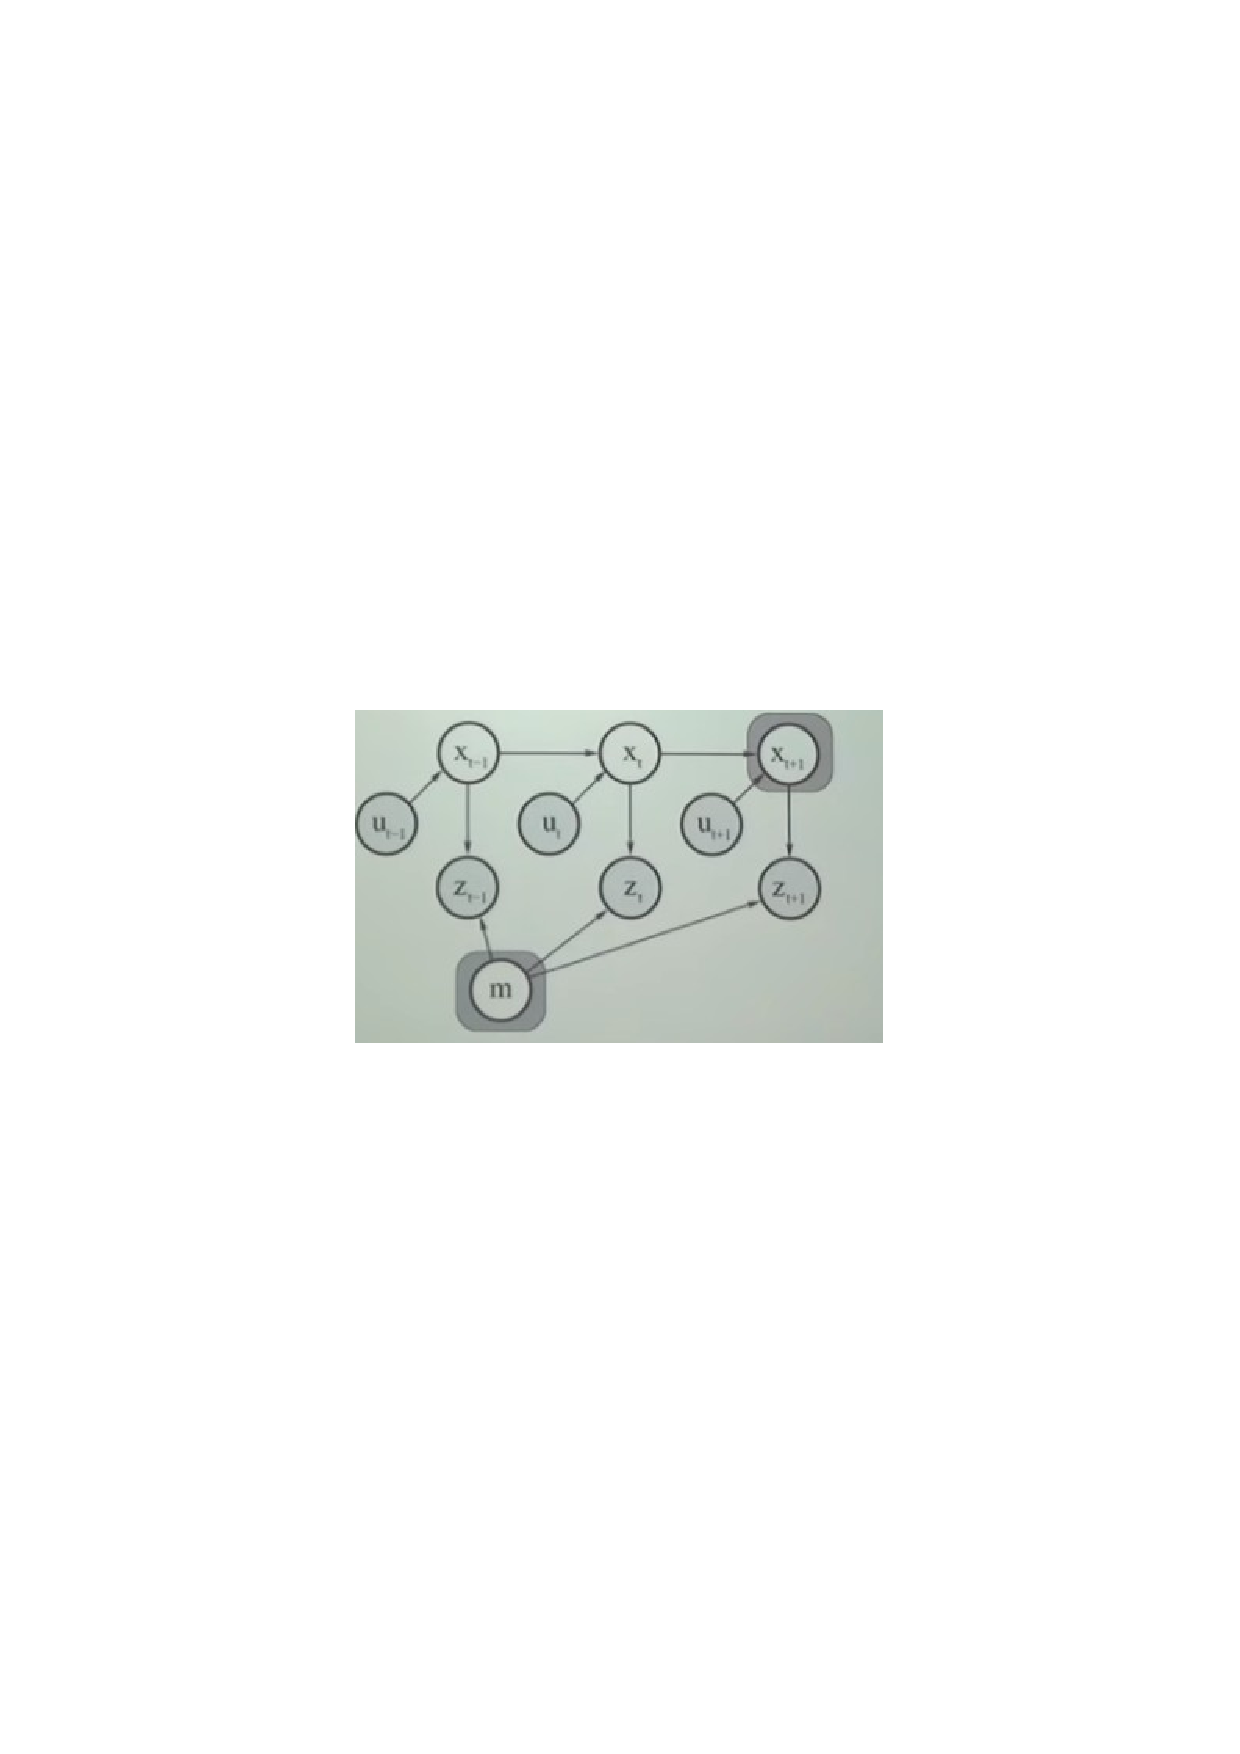
\includegraphics[scale=0.8]{Online_SLAM.pdf}
\end{frame}

\begin{frame}{Motion and Observation model}\vspace{5pt}
\centering
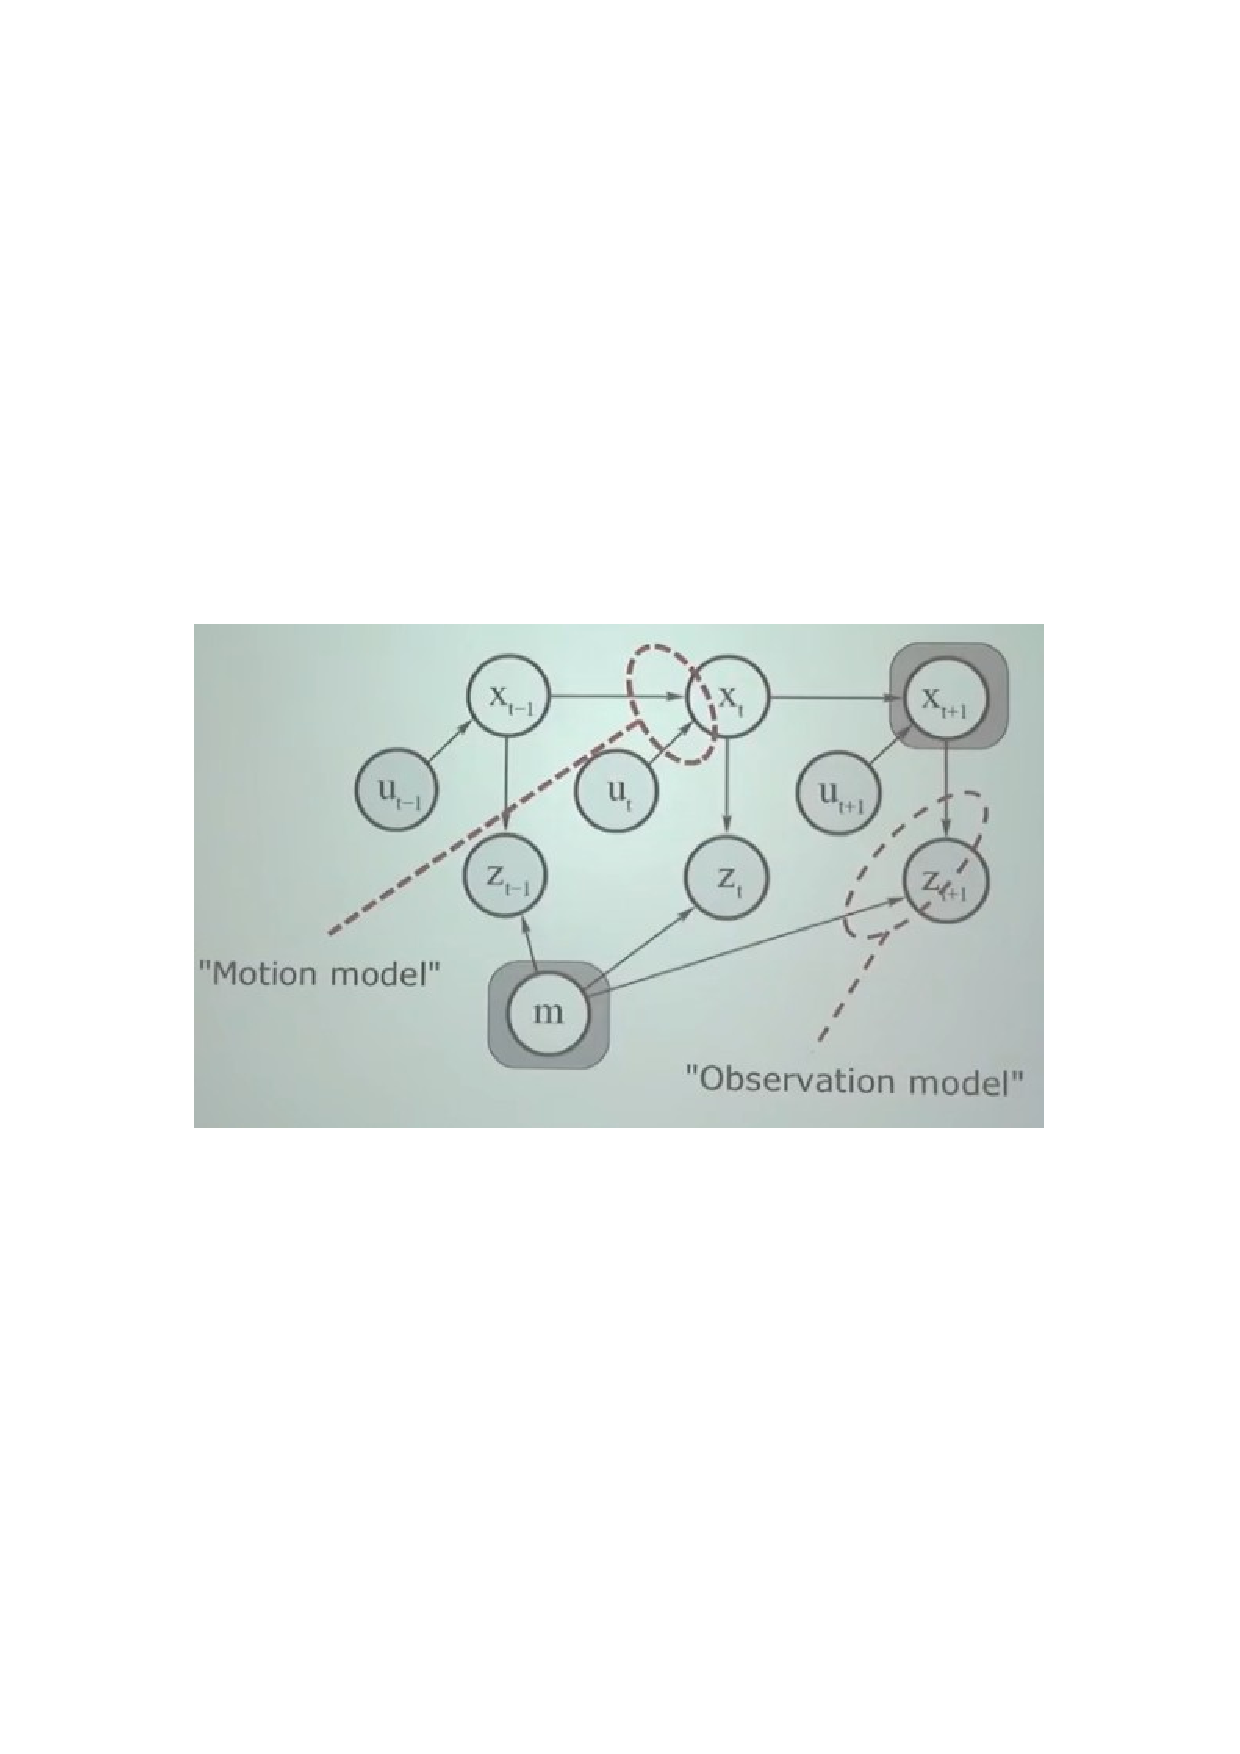
\includegraphics[scale=0.7]{model.pdf}
\end{frame}

\begin{frame}{Motion Model}
\begin{itemize}
\item The motion model describes the relative motion of the robot
\end{itemize}
\centering
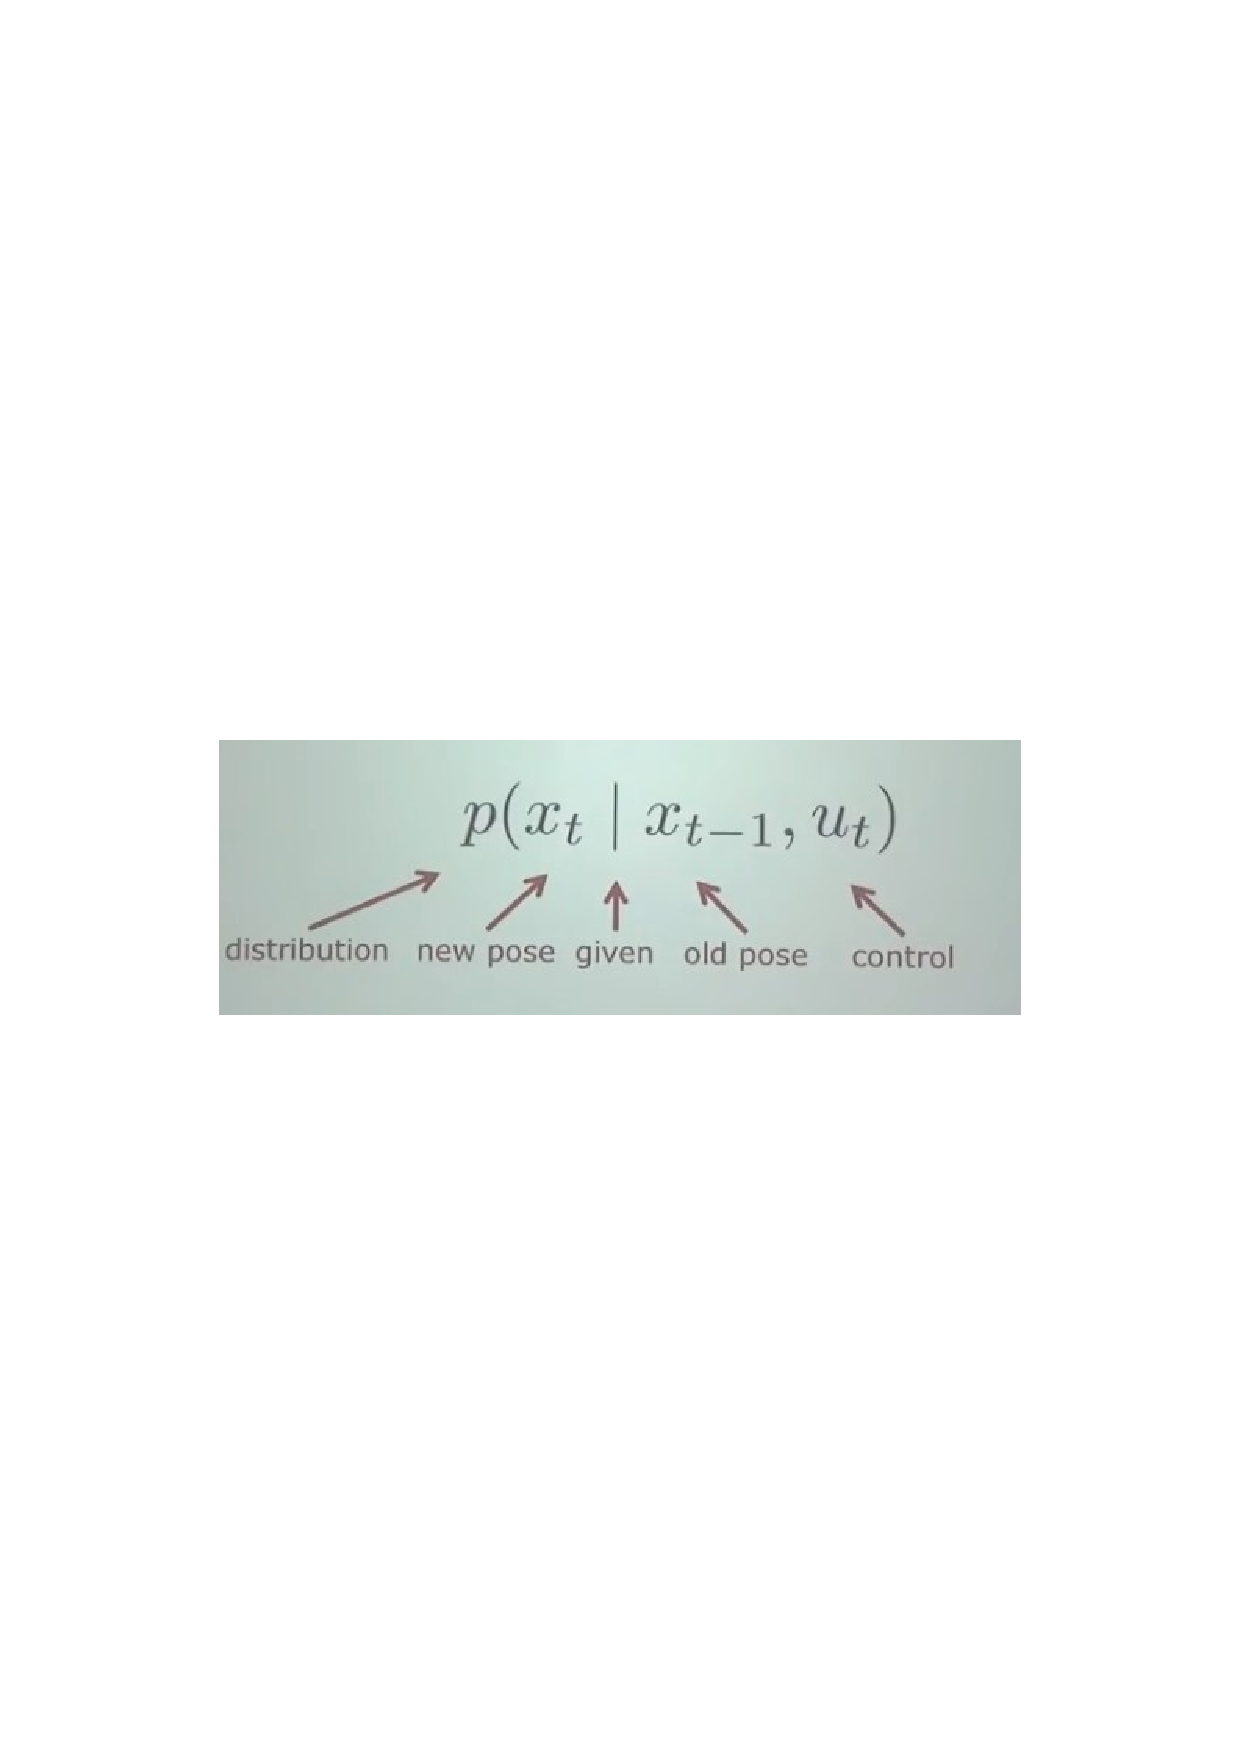
\includegraphics[scale=0.5]{motion_model.pdf}
\end{frame}

\begin{frame}{Observation Model}
\begin{itemize}
\item The observation or sensor model relates measurements with the robot's pose
\end{itemize}
\centering
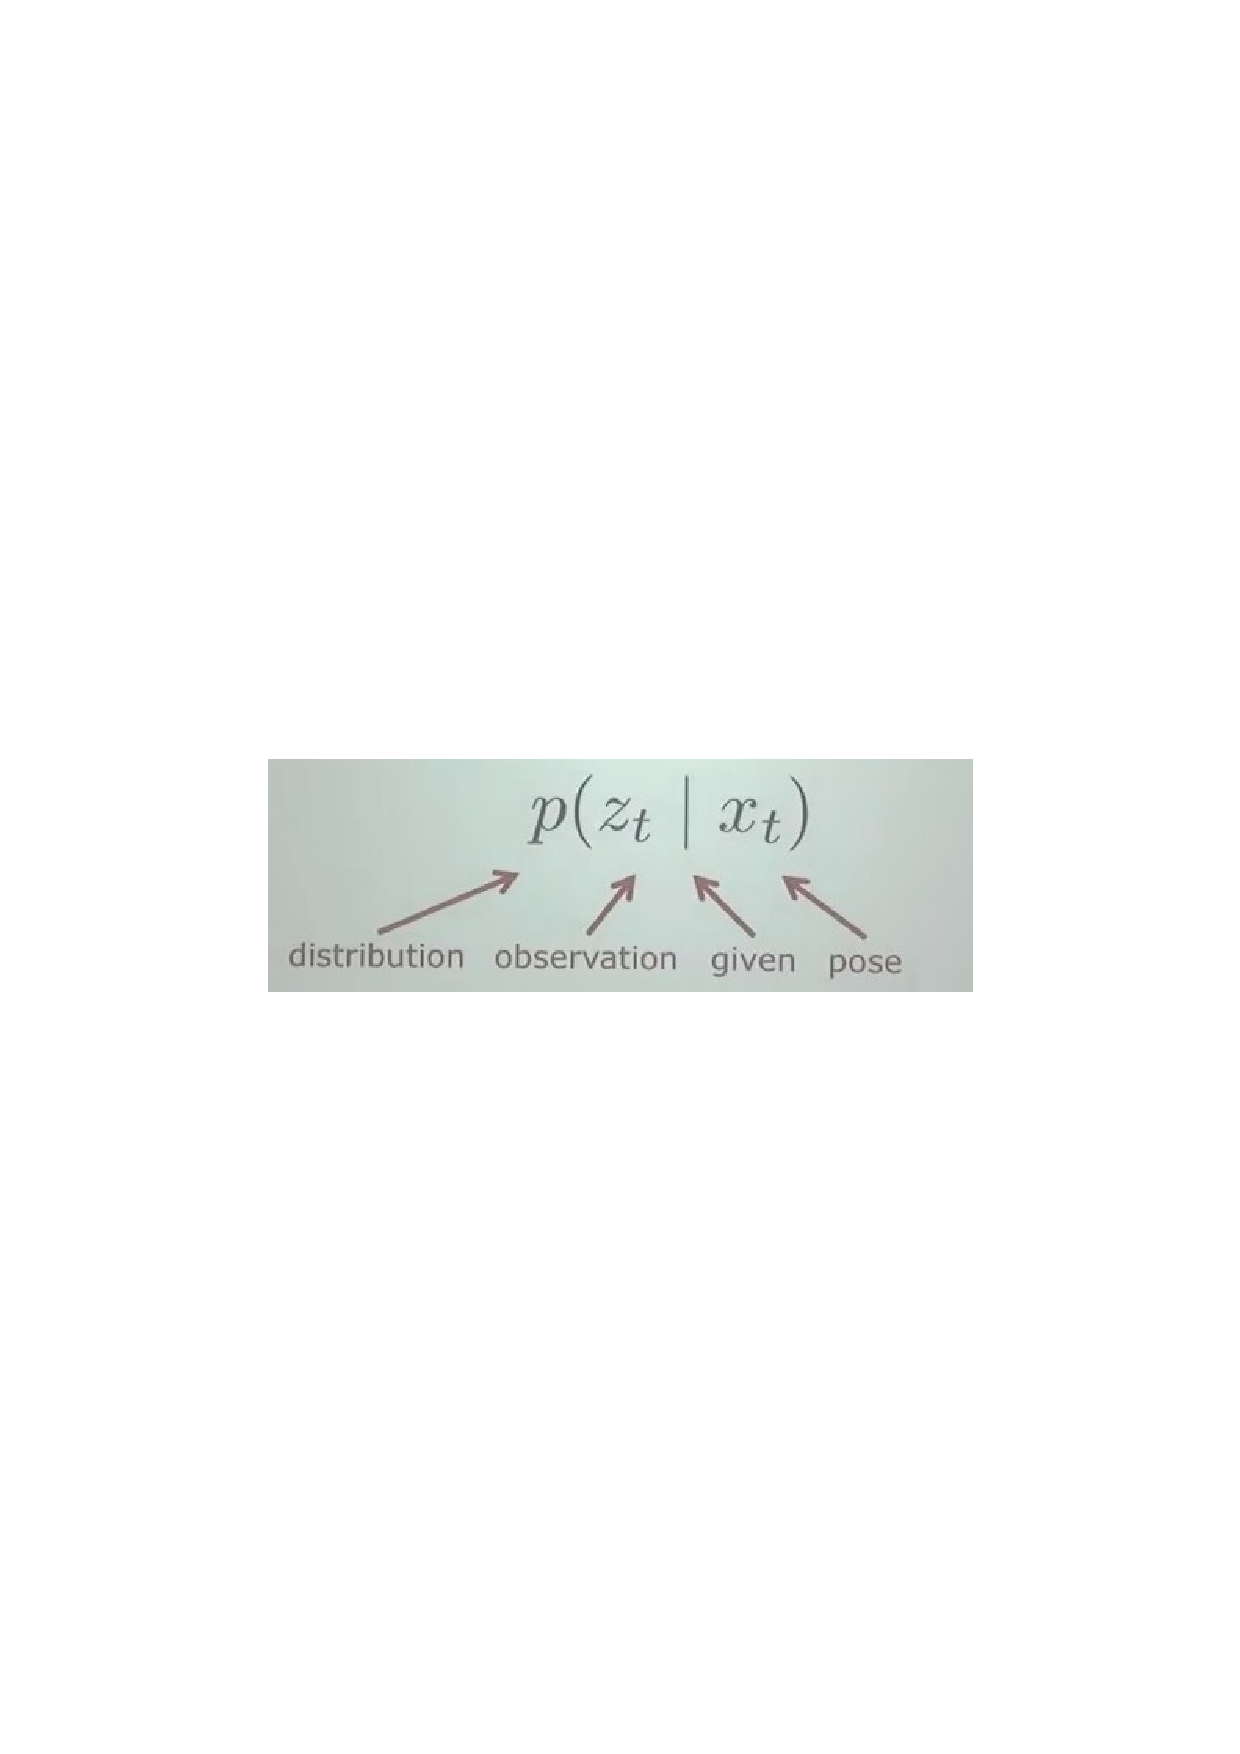
\includegraphics[scale=0.5]{observation_model.pdf}
\end{frame}

\begin{frame}{Progress}
\textbf{Three Main SLAM Paradigms}
\begin{multicols}{3}
\begin{tcolorbox}[colback=blue!5!white,colframe=red!75!black]
\centering
Kalman\\
filter
\end{tcolorbox}
\begin{tcolorbox}[colback=blue!5!white,colframe=blue!75!black]
\centering
Particle\\
filter
\end{tcolorbox}
\begin{tcolorbox}[colback=blue!5!white,colframe=blue!75!black]
\centering
Graph-based filter
\end{tcolorbox}
\end{multicols}
\end{frame}

\begin{frame}[t]{EKF SLAM: Filter Cycle}
\begin{enumerate}[1]
\item State prediction
\item Measurement prediction
\item Measurement
\item Data association
\item Update
\end{enumerate}
\end{frame}

\begin{frame}{EKF SLAM Simulation}
\centering
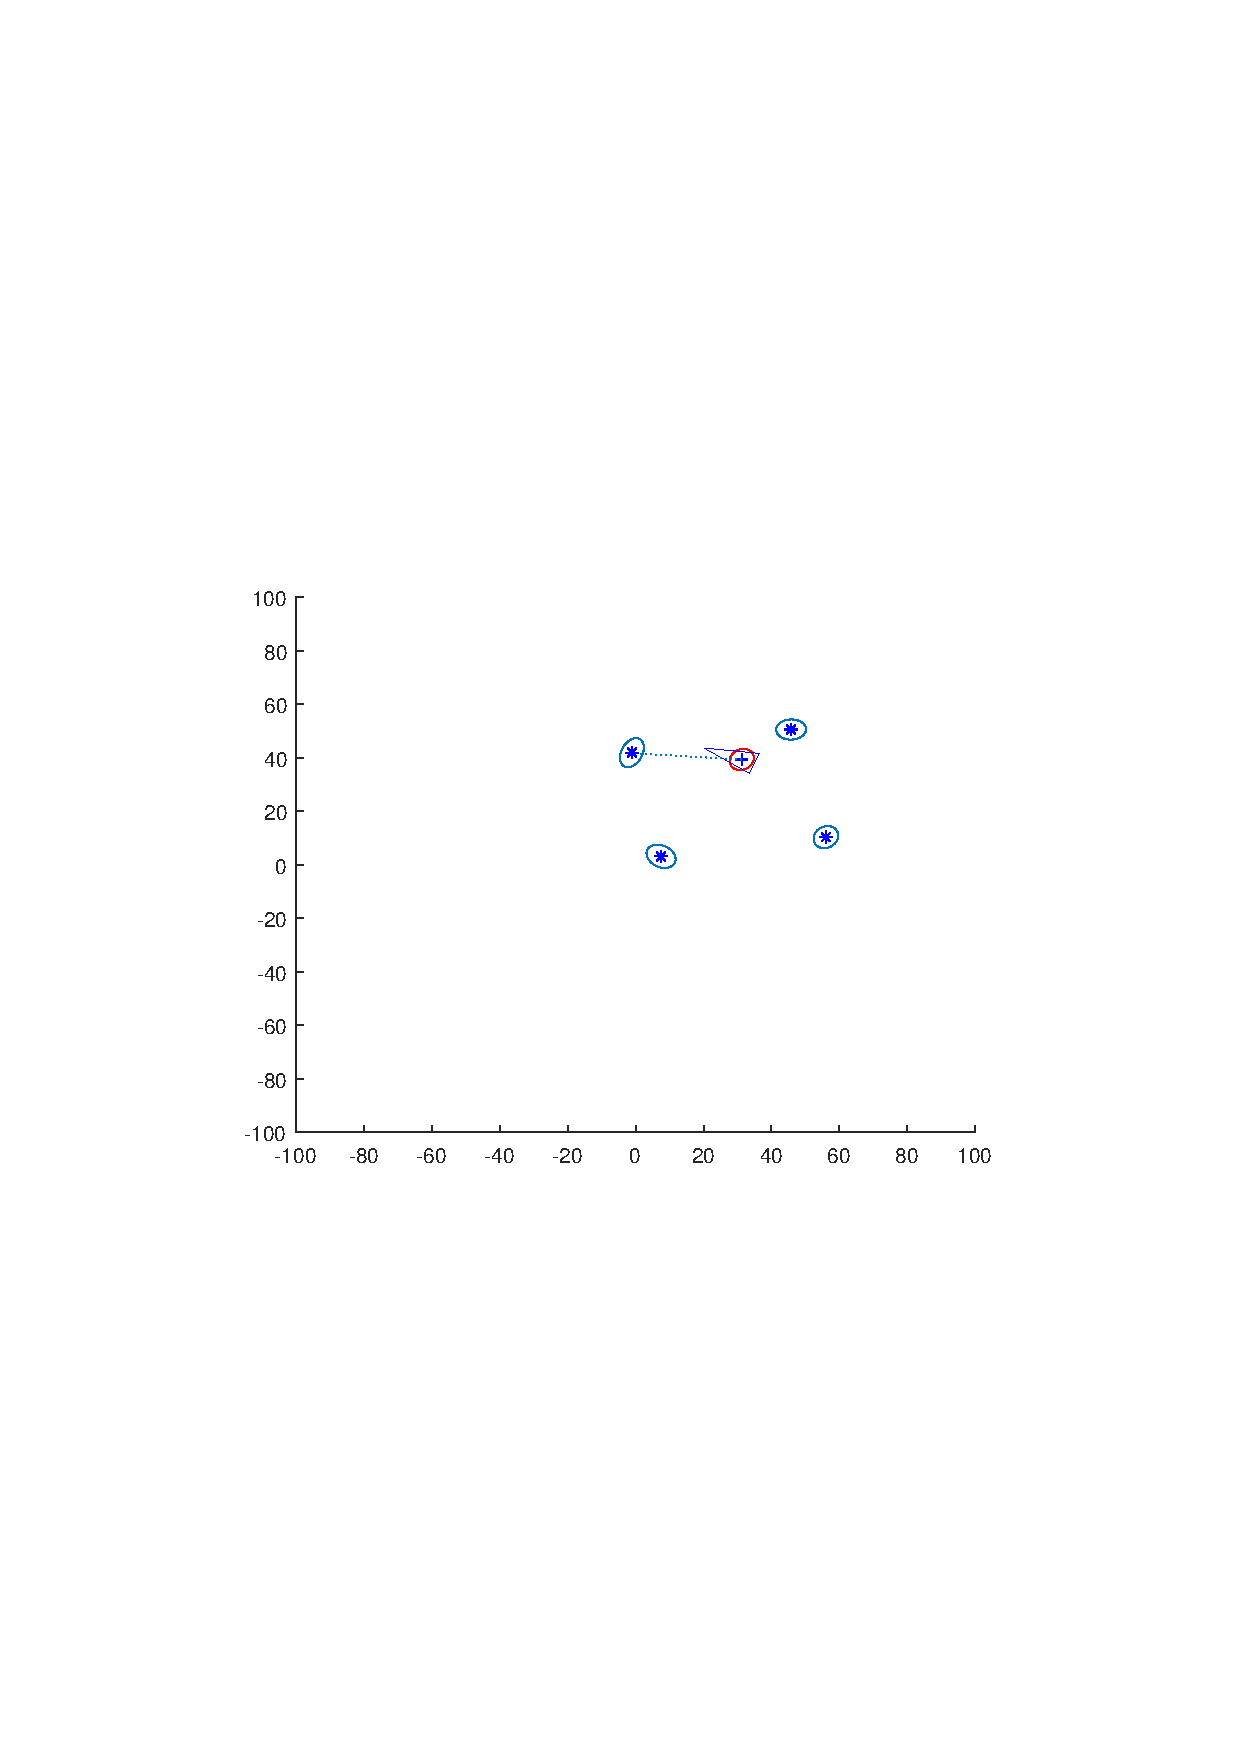
\includegraphics[scale=0.75]{SLAM_simulation.pdf}
\end{frame}

\begin{frame}{Goal and Application}
I can build a small autonomous car in the specific space, and help me with cleaning. 
\end{frame}
\end{document}
